\chapter{Mediciones y Resultados}
Se conectan entonces ambos circuitos en la placa \textit{Electronics Explorer}. Debido a las limitaciones del dispositivo, se utilizó una tensión de alimentación de $V_{CC} = 9V$ tanto para el par Darlington como para la carga activa.
A su vez se utiliza el generador arbitrario de funciones para inyectar una señal de $500 mV$ a una frecuencia de $10kHz$ con el objetivo de medir la respuesta del circuito a pequeñas señales. En principio se plantea una señal de $50 mV$, pero debido a una considerable cantidad de ruido en la medición se imposibilita la realización precisa de la misma del sistema.
Requiriendo entonces una mayor entrada, esta se incrementa cuidando no perder la linealidad de la respuesta hasta el valor propuesto previamente.
La medición de la ganancia de corriente no es realizable. Principalmente debido a que la corriente de entrada es menor de la medible con el equipo previsto, sin afectar el comportamiento del circuito.

\section{Circuito Construido}
Se presenta una imagen anotada del circuito con carga activa en la imagen \ref{fig: foto circuito carga activa}. Luego se alterna la conexión en el emisor de $Q2$ entre dos resistencias en serie representando $R_E$ y en la fuente de corriente espejo conformado por los MOS-FET del lado derecho. Como $900 \Omega$ no es un valor estándar, se conecta en serie una resistencia de $680 \Omega$ y una de $220 \Omega$.

\begin{figure}[ht]
    \centering
    \includegraphics[width = 0.8\textwidth]{4_medicion/figs/fotos circuito/Carga Activa editada.jpg}
    \caption{Imagen anotada del circuito con carga activa}\label{fig: foto circuito carga activa}
\end{figure}
%%Nose si dejarla esta, es igual a la anterior pero con 2 resistencias
\begin{figure}[ht]
    \centering
    \includegraphics[scale = 0.05]{4_medicion/figs/fotos circuito/Carga Pasiva.jpg}
    \caption{Imagen del circuito con carga pasiva}\label{fig: foto circuito carga pasiva}
\end{figure}


\section{Mediciones}

Se midieron los parámetros de del circuito tanto para el uso de una carga pasiva como de una carga activa.

\subsection{Caracterización de fuente de corriente}

Fue necesario en principio encontrar el valor de $I_O$ de la fuente de corriente. Al ser un componente real, no se puede esperar que ambos transistores n-MOS compartan el mismo valor de $\frac{W}{L}$, por lo que la relación de corrientes escrita en \ref{eq:io func iref} no es unitaria.
Como se requiere un valor especifico de $I_O$ para la tener una comparación justa entre usar o no una carga activa, se utilizó una resistencia variable como $R_{ref}$ y se la varió hasta que en la salida la corriente sea de los $8,6 mA$ requeridos. Esta calibración se realizó con la salida de la fuente de corriente conectada a $V_{CC}$ y una resistencia de referencia de $1k\Omega$.

\subsection{Polarización}

Para verificar el correcto funcionamiento del par Darlington, y su correspondencia con la teoría, se realizaron mediciones de la polarización del mismo. Caracterizada por la tabla \ref{table:pola medida}. Las caídas de tensión se midieron con dos puntas del osciloscopio y calculando la diferencia entre los canales con el canal matemático.

Por otro lado, para las corrientes se midió la diferencia de potencial a través de una resistencia de referencia de $100 \Omega$ de tolerancia $1\%$, y se la dividió por su valor nominal.

\begin{table}[ht]
    \centering
    \begin{tabular}{|l|r|r|r|r|}
        \hline
        \multirow{2}{*}{} & \multicolumn{2}{c|}{Carga Pasiva} & \multicolumn{2}{c|}{Carga Activa} \\ \cline{2-5} 
         & $Q_1$ & $Q_2$ & $Q_1$ & $Q_2$ \\ \hline

        $I_{CQ} (\si{\ampere})$ & $133 \si{\micro}$& $9.039\si{\milli}$ & $94.7 \si{\micro}$& $10.55\si{\milli}$\\
        $V_{CE} (\si{\volt})$   & $0.429$            & $1.209$ & $0.542$ & $1.23$ \\ \hline       
    \end{tabular}
    \caption{Medición polarización de cada transistor}
    \label{table:pola medida}
\end{table}

A partir de estos datos, se pudo trazar comparaciones con la tabla \ref{tab:vals_teo} conteniendo la polarización teórica de cada elemento. En primer lugar se observó una diferencia porcentual alta entre las $I_{CQ1}$ con carga pasiva y activa, de un $50\%$ de diferencia. No se consideró que esta diferencia afectara al circuito críticamente, dado los extremadamente bajos niveles de corriente. Además, esto no presentó una diferencia igual de crítica en la $I_{CQ2}$.

Sin embargo, sigue siendo un margen de error considerable, dado que no coincide con las aproximaciones teóricas de las ecuaciones \eqref{eq:pol_I_E2} y \eqref{eq:pol icq}. (Por el momento aún estamos intentando encontrar una causa posible a esta discrepancia).
%(NO SE ME OCURRE OTRA COSA, A USTEDES????)

Por otro lado las tensiones colector-emisor con ambas cargas en $Q_2$ se acercan a lo estimado teóricamente. Y las corrientes de colector presentan una diferencia de unos pocos mili amperes con la teórica. Esto es atribuible al hecho de que como se trata de transistores reales, su parámetro de ganancia de corriente se encuentra dentro de un amplio rango de valores. Muy probablemente el que se toma para el calculo teórico no es el que presentan los transistores en la realidad.


\subsection{Ganancia de Tensión}

En las tablas \ref{table:comp av} y \ref{table:comp avs} se muestran los resultados para $\Delta_V$ y $\Delta_{Vs}$ en ambas configuraciones contrastando con lo simulado y lo estimado teóricamente.
Se utilizó una $R_g$ de $50\Omega$, ya que no se encuentra disponible el valor de la impedancia de salida del generador de funciones del \textit{Electronics Explorer}.

\begin{table}[ht]
    \centering
    \begin{tabular}{|l|l|l|l|}
    \hline
    $\Delta_V $  & Medida   & Teórica  & Simulación \\ \hline
    Carga Pasiva & $0.967$  & $0,9904$ &  $0.9437$       \\ \hline
    Carga Activa & $0.983$  & $0,9992$ &  $0.9514$          \\ \hline
    \end{tabular}
    \caption{Tabla comparación $\Delta_V$}\label{table:comp av}
\end{table}

\begin{table}[ht]
    \centering
    \begin{tabular}{|l|l|l|l|}
    \hline
    $\Delta_{VS} $  & Medida   & Teórica  & Simulación \\ \hline
    Carga Pasiva & $0.929$  & $0,943$ &  $XX$       \\ \hline
    Carga Activa & $0.942$  & $0,9943$ &  $XX$          \\ \hline
    \end{tabular}
    \caption{Tabla comparación $\Delta_{VS}$}\label{table:comp avs}
\end{table}

Como es de esperar no se midió exactamente lo mismo a lo estimado el la teoría. Aún así, las mediciones se encuentran en un margen de tolerancia aceptable. 
Es evidente que la carga activa mejora el rendimiento del amplificador. Ya que para pequeñas señales, el $Q_2$ verá una mayor resistencia en su emisor mejorando $R_D$ pero manteniendo una similar polarización. 
También se manifiesta la forma en la que $R_S$ degrada el valor de la ganancia, en donde es más perceptible es con la carga activa. 

Se presenta en las figuras \ref{fig:Av oscilo}, el contraste entre formas de onda de salida y entrada para ambas cargas.


\begin{figure}[ht]
\begin{subfigure}{.45\textwidth}
  \centering
  % include first image
  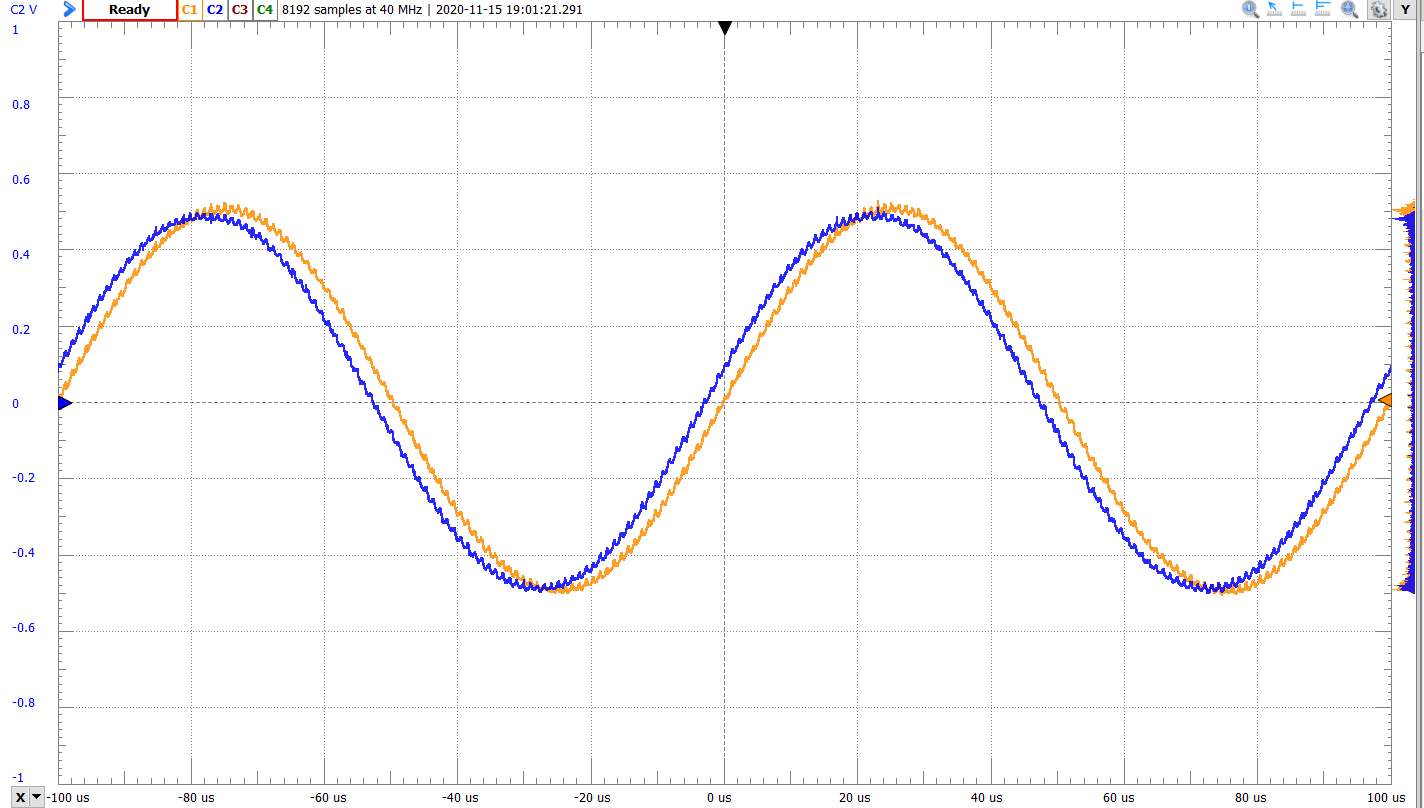
\includegraphics[width=.8\linewidth]{4_medicion/figs/2 pasada/Pasiva/carga pasiva Av c1 entrada c2 salida editada.png}  
  \caption{Carga Pasiva}
  \label{fig:Av carga pasiva}
\end{subfigure}
\begin{subfigure}{.45\textwidth}
  \centering
  % include second image
  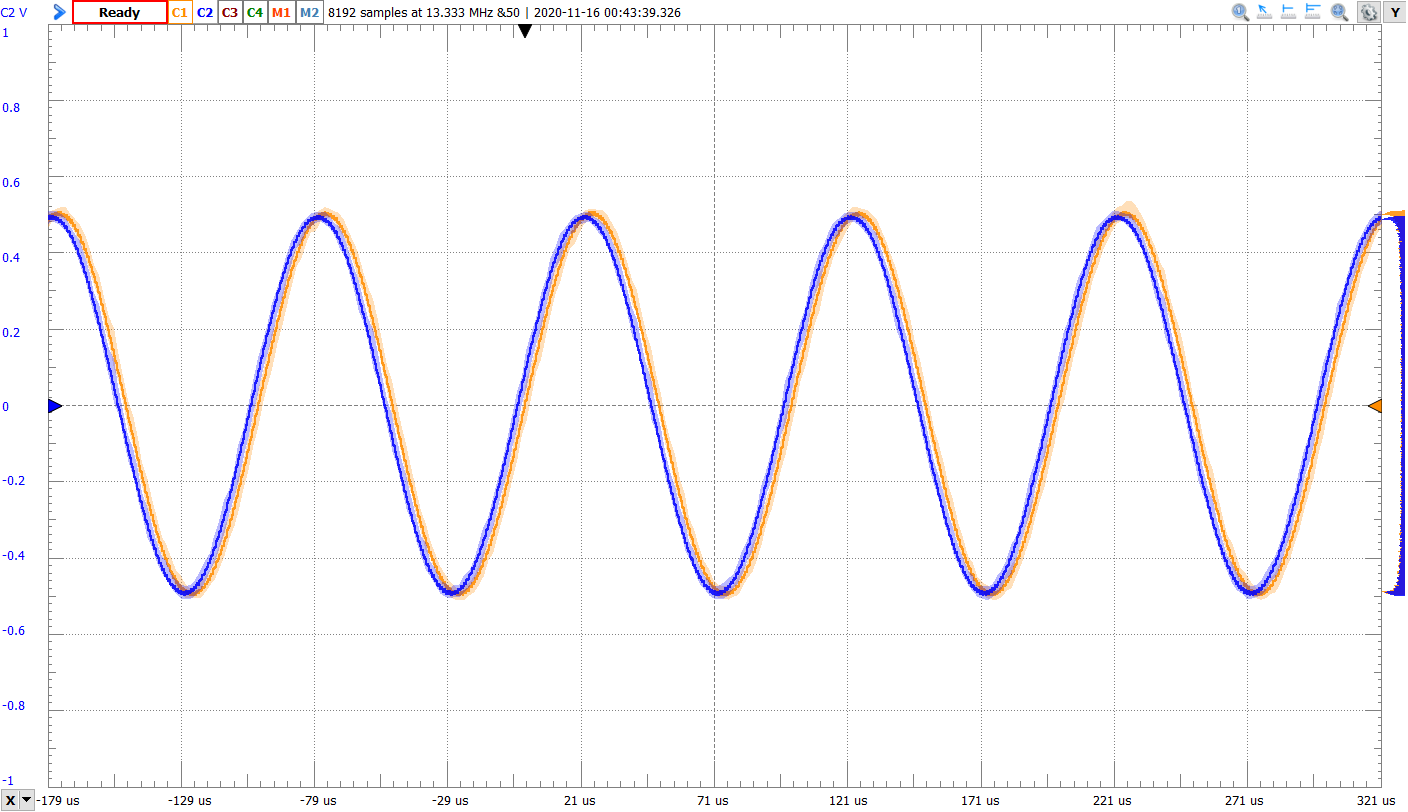
\includegraphics[width=.8\linewidth]{4_medicion/figs/2 pasada/Activa/carga activa Av c1 entrada c2 salida.png}  
  \caption{Carga Activa}
  \label{fig:Av carga activa}
\end{subfigure}
\caption{Adquisición Osciloscopio}
\label{fig:Av oscilo}
\end{figure}

\subsection{Impedancias de Entrada y Salida}

El procedimiento que se empleó para medir la impedancia de entrada consistió en insertar una resistencia de referencia de $1 k\Omega$ con tolerancia $1\%$ entre el generador de ondas y el capacitor de desacople en la base de $Q_1$. Se eligió este valor ya que es comparable al estimado teóricamente.

Midiendo la caída de tensión en esta y dividiendo por su valor nominal, se calculó la corriente que entra a la base del transistor para pequeñas señales. Luego el cociente entre la tensión de entrada a la base, y la corriente previamente calculada se estimó el valor de interés. Esta medición correspondió a la impedancia de entrada del amplificador, por lo que el valor no es alto como se esperaría del par Darlington.

Ya que esta se encuentra en paralelo con $R_B$, la cual es mucho menor a la calculada para el par Darlington sin considerar su periferia. Llevando entonces al bajo valor encontrado en la práctica.
Se realiza el mismo procedimiento para la carga activa y pasiva, por mas que se espera un resultado muy similar. En la tabla \ref{table:Ri comp}, se contrastó lo medido,simulado y calculado teóricamente.

\begin{table}[ht]
    \centering
    \begin{tabular}{|l|l|l|l|}
    \hline
    $r_{ia}$     & Medida       & Teórica         & Simulación \\ \hline
    Carga Pasiva & $1013\Omega$ & $1000\Omega $   &  $XX $          \\ \hline
    Carga Activa & $1018\Omega$ & $1000\Omega $  &  $XX $          \\ \hline
    \end{tabular}
    \caption{Comparación impedancia de entrada}\label{table:Ri comp}
\end{table}

Se observó entonces que lo medido y lo calculado presentaron una semejanza notable. Justificando entonces el razonamiento de que $R_B$ empeora marcadamente la impedancia de entrada del amplificador.

Para la impedancia de salida se realizó una técnica prevista en el material didáctico de la cátedra que consistió en medir la tensión a la salida del amplificador a circuito abierto (carga infinita),denominada $V_{open}$. Luego se introdujo una carga $R_L$ y se midió la tensión $V_L$ a través de la misma.

Contando con estos valores se empleó la ecuación \eqref{eq:zout teor}, encontrando así un valor para la impedancia de salida, caracterizadas en la tabla \ref{table:Ro comp}

\begin{equation}
    R_O = R_L(\frac{V_{open}}{V_L}-1)
    \label{eq:zout teor}
\end{equation}

\begin{table}[ht]
    \centering
    \begin{tabular}{|l|l|l|l|}
    \hline
    $r_{oa}$     & Medida     & Teórica         & Simulación \\ \hline
    Carga Pasiva & $23\Omega$ & $5,91\Omega $   &  $XX $          \\ \hline
    Carga Activa & $18\Omega$ &  $5,91\Omega $  &  $XX $          \\ \hline
    \end{tabular}
    \caption{Comparación impedancia de Salida}\label{table:Ro comp}
\end{table}

Con una diferencia de unos pocos $\Omega$ se volvió a presenciar una similitud entre la práctica y la teoría. Estos valores de resistencia de salida son una virtud de este circuito, siempre se busca que sea baja a fin de no cargar ni afectar etapas posteriores a la misma. Especialmente en un seguidor de emisor o buffer.

\subsection{Respuesta en Frecuencia}

La respuesta en frecuencia se midió usando el \textit{Network Analizer} incluido en el equipo de medición. Debido a su bajo ancho de banda se dificulta medir el polo de alta, ya que su frecuenciia excede el límite de medición de $10 MHz$. No obstante una década antes del polo previsto se pudo observar un cambio de fase, como es de esperar.
El polo de baja se observó claramente en el rango determinado. En las figuras \ref{fig:frec carga pasiva} y \ref{fig:frec carga activa} se muestra la respuesta medida.

%\begin{figure}[ht]
%    \begin{subfigure}{.45\textwidth}
%      \centering
%      % include first image
%      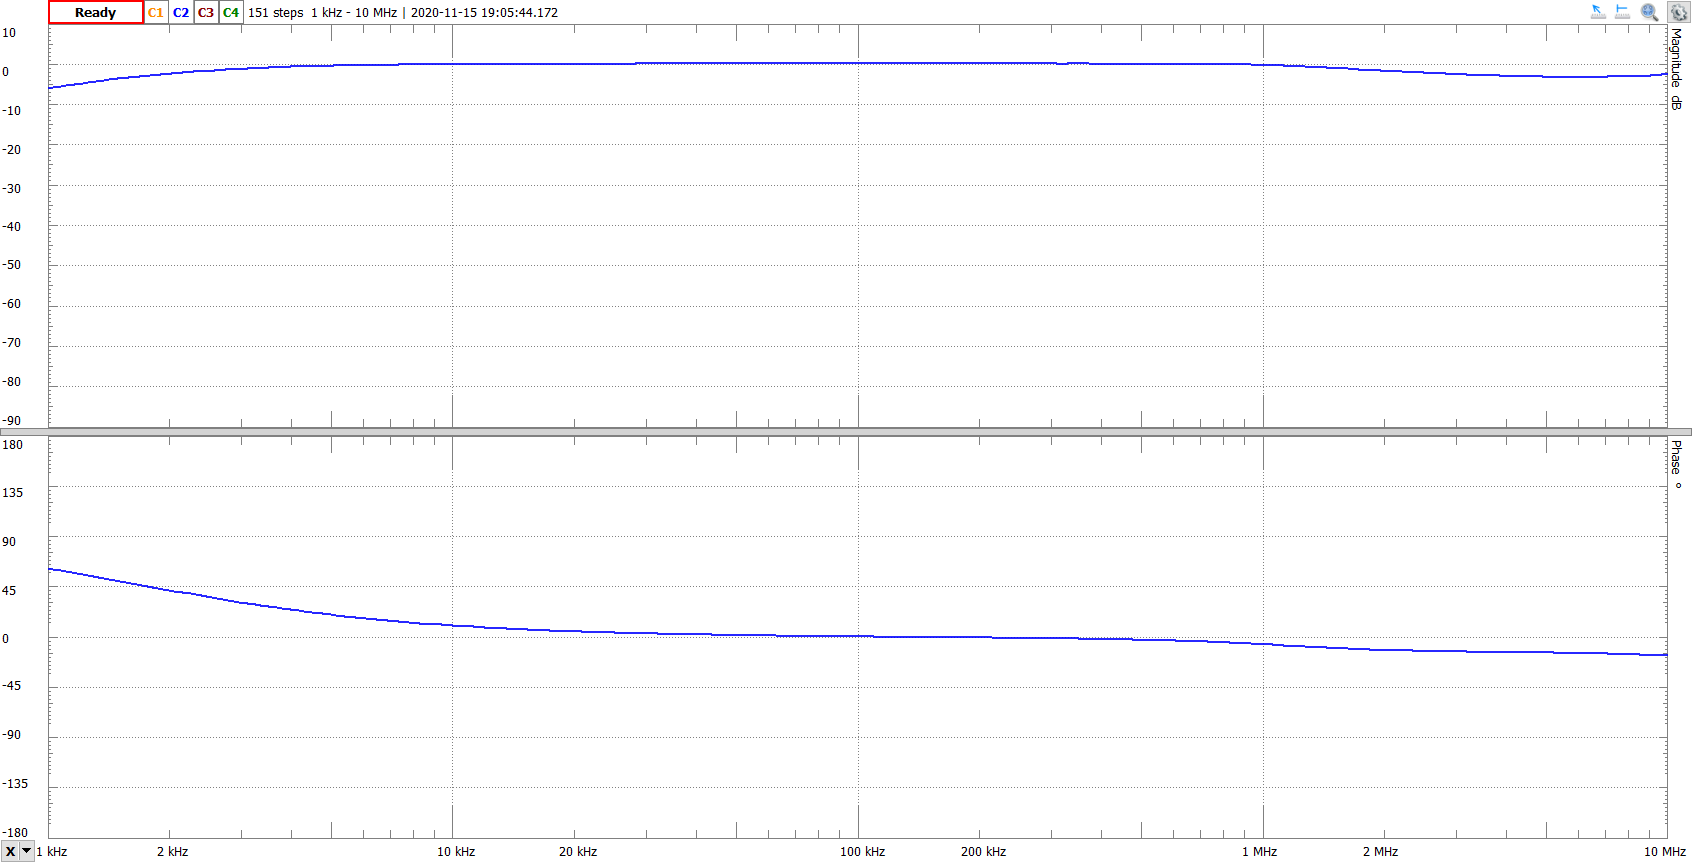
\includegraphics[width=.8\linewidth]{4_medicion/figs/2 pasada/Pasiva/resp frec.png}  
%      \caption{Carga Pasiva}
%      \label{fig:frec carga pasiva}
 %   \end{subfigure}
  %  \begin{subfigure}{.45\textwidth}
   %   \centering
  % include second image
%     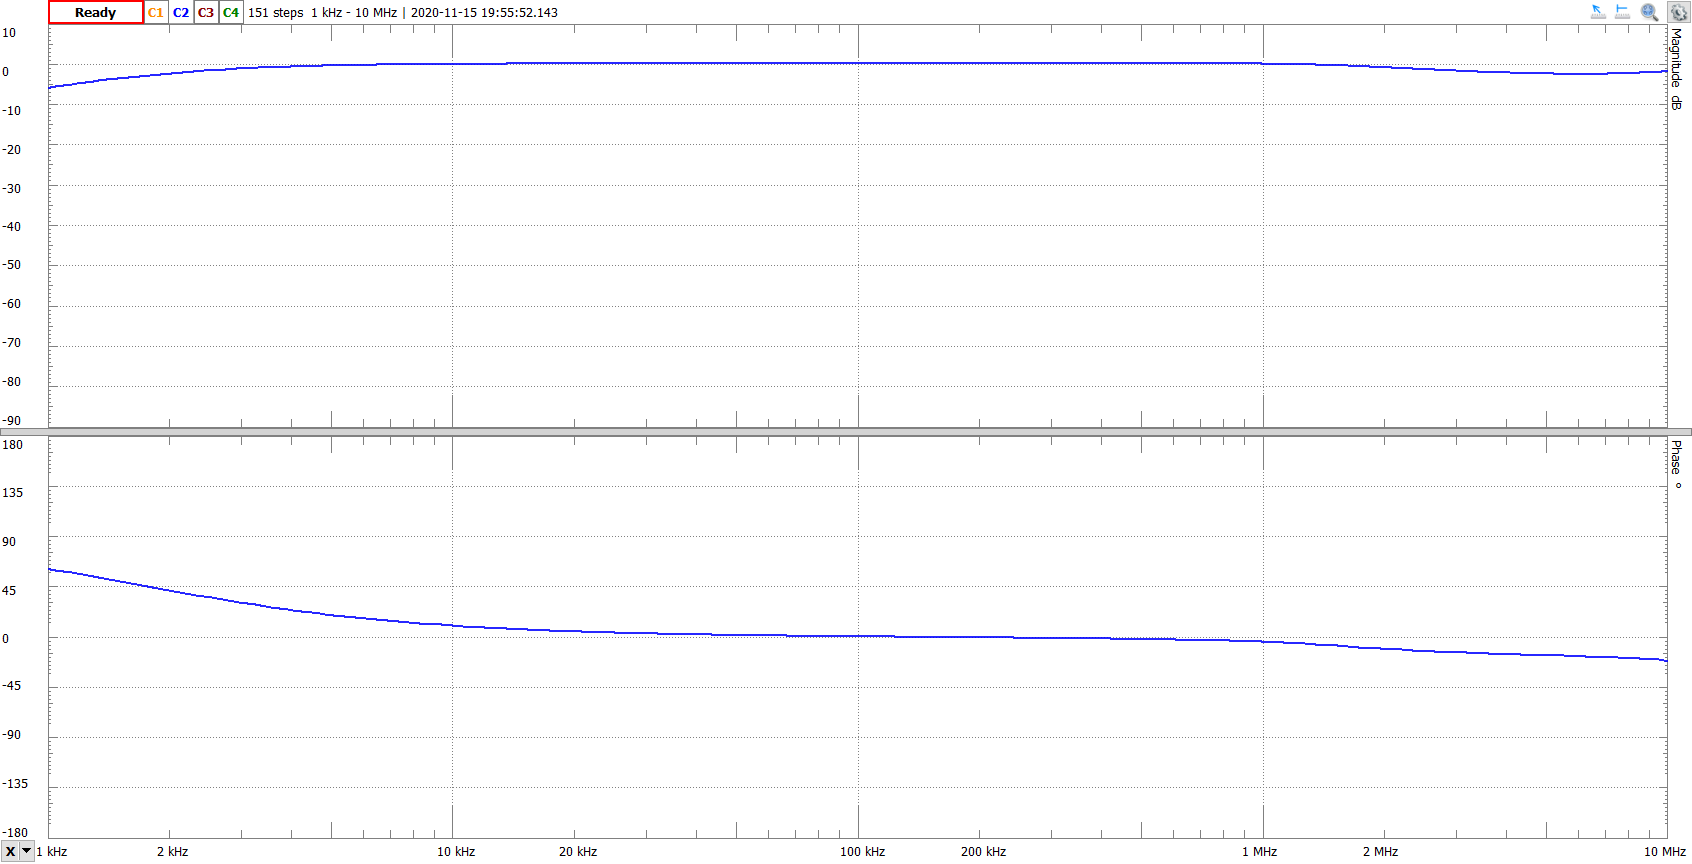
\includegraphics[width=.8\linewidth]{4_medicion/figs/2 pasada/Activa/respfrec.png}  
%      \caption{Carga Activa}
%      \label{fig:frec carga activa}
%    \end{subfigure}
%    \caption{Respuesta en frecuencia}
%    \label{fig:resp frec oscilo}
%    \end{figure}


\begin{figure}[ht]
    \centering
    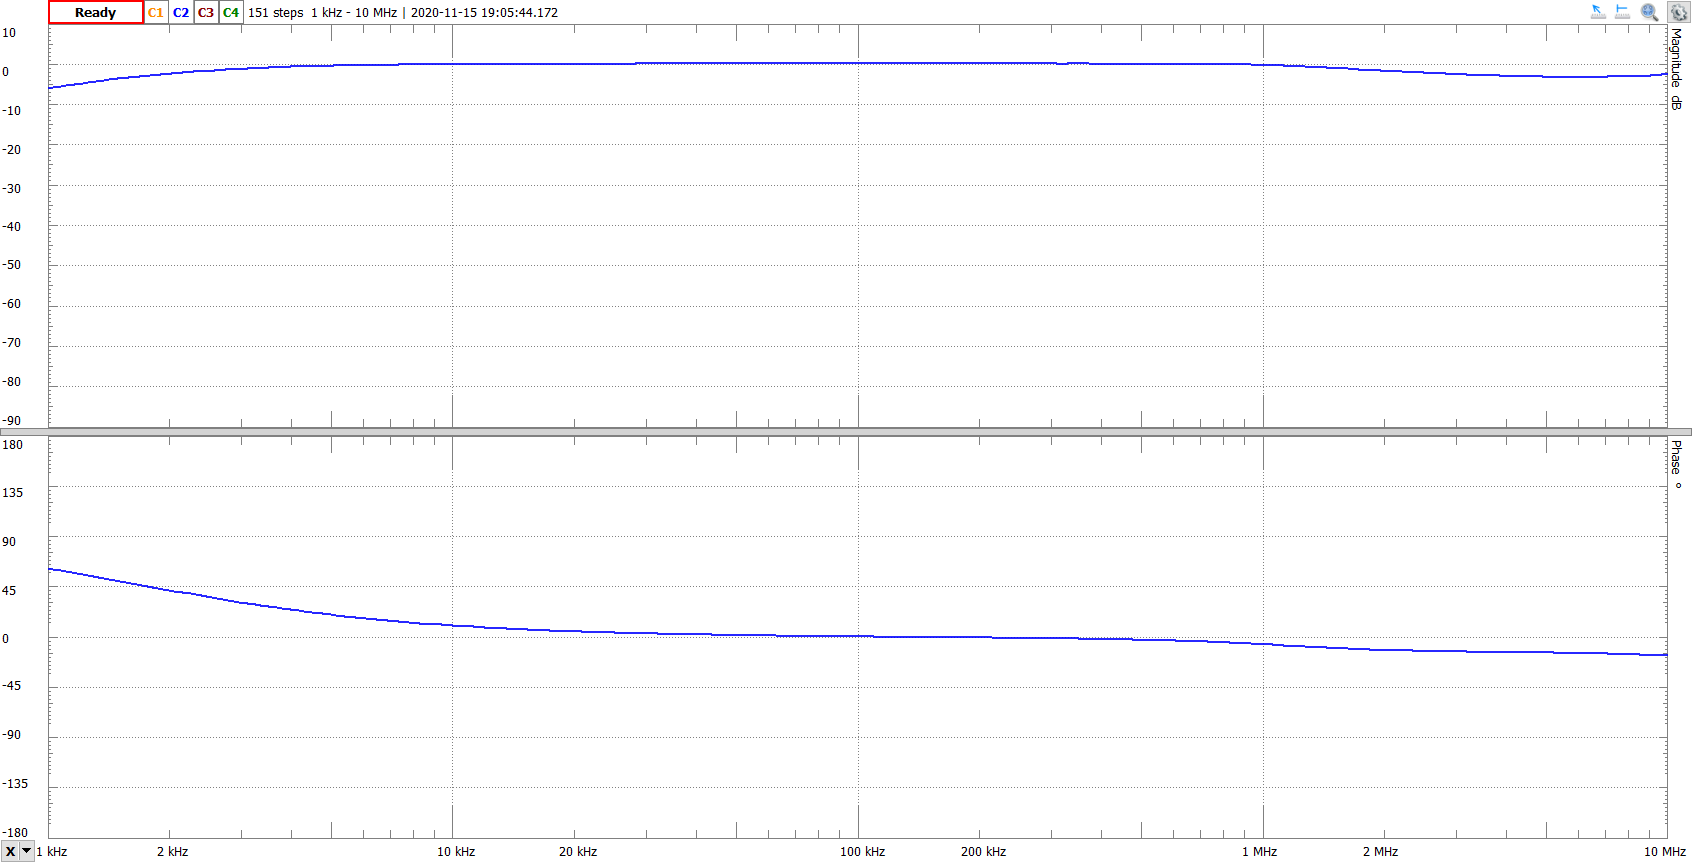
\includegraphics[width = 0.8\textwidth]{4_medicion/figs/2 pasada/Pasiva/resp frec.png}
    \caption{Carga Pasiva}
    \label{fig:frec carga pasiva}
\end{figure}

\begin{figure}[ht]
    \centering
    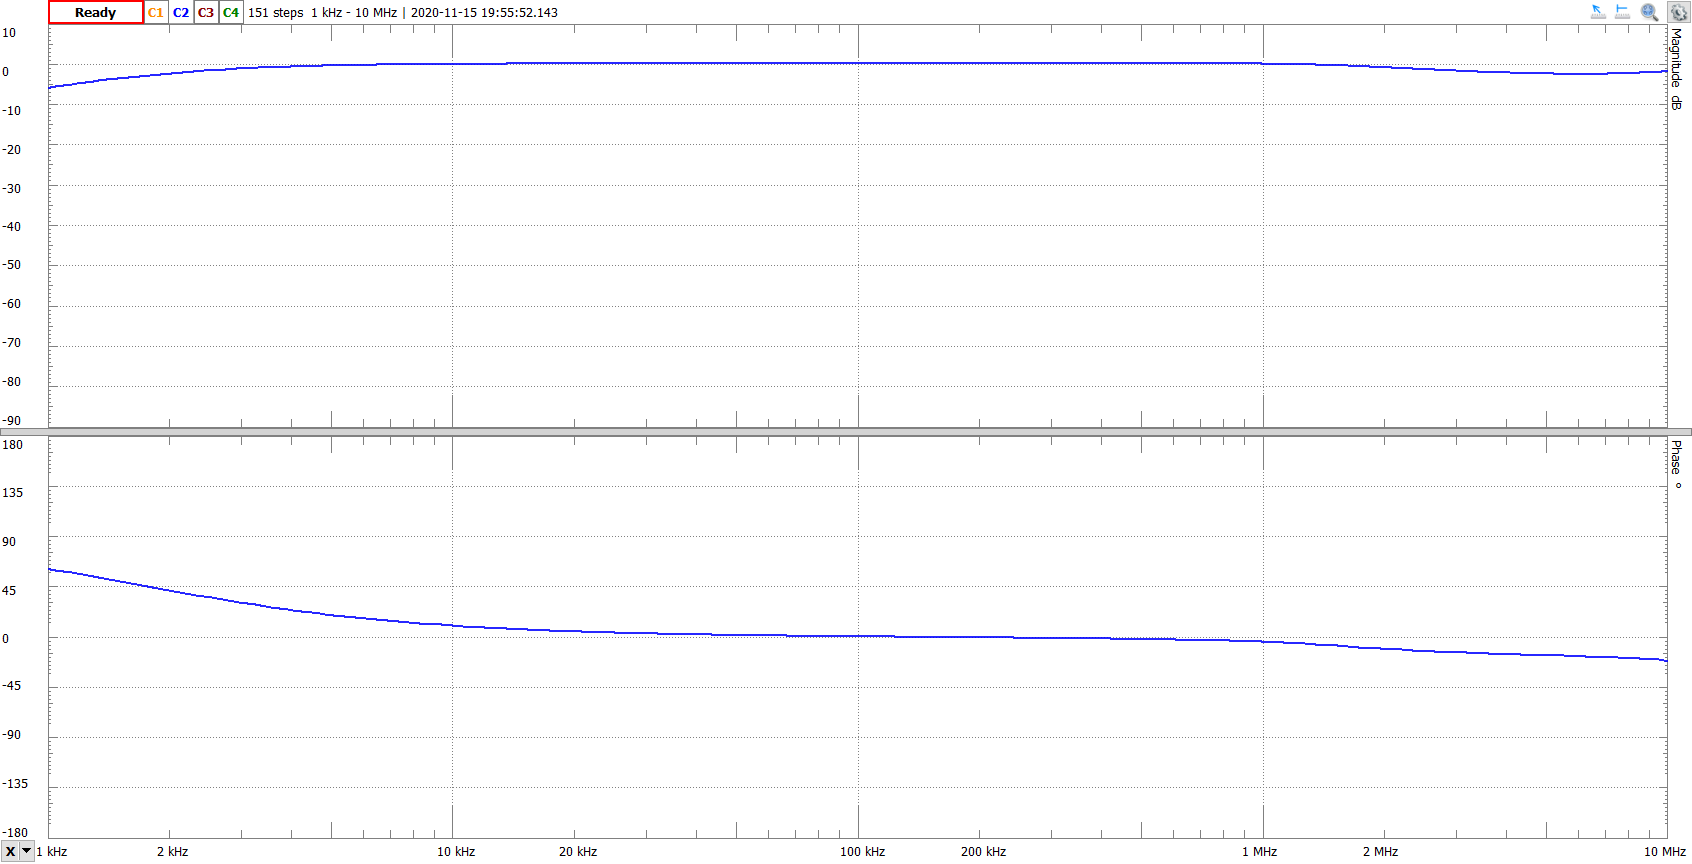
\includegraphics[width = 0.8\textwidth]{4_medicion/figs/2 pasada/Activa/respfrec.png}
    \caption{Carga Activa}
    \label{fig:frec carga activa}
\end{figure}